\documentclass[12pt,titlepage,a4paper]{report}
% Texte
\usepackage[utf8]{inputenc}
\usepackage[T1]{fontenc}
\usepackage[french]{babel}
\usepackage{lmodern}
\usepackage{enumitem}
\usepackage{minted}
% Pour les checkmarks
\usepackage{pifont}
\usepackage{amssymb}
% Pour des \hline en gras
\usepackage{makecell}
% Numéroter les chapitres à partir de chaque début de partie
\makeatletter\@addtoreset{chapter}{part}\makeatother

% Mise en page
\usepackage{url}
\usepackage[top=2.1cm,bottom=2cm,left=1cm,right=1cm]{geometry}
\usepackage{hyperref}
\hypersetup{
    colorlinks=false,
    pdfborder={0 0 0},
}
\usepackage{multirow}

% TOC
\usepackage[french]{minitoc}
\setcounter{tocdepth}{2}
\setcounter{minitocdepth}{2}
\setlength{\mtcindent}{0pt}

% Images
\usepackage{float}
\usepackage{wrapfig}
\usepackage{graphicx}
% Pour inclure des pages PDF
\usepackage[final]{pdfpages}

% Couverture
\usepackage{templateINSA}
\initINSA

\title{BD Université}
\author{Manon \bsc{Ansart}\\ Antoine \bsc{Augusti}}

\renewcommand\soustitre{Rapport de projet}
\renewcommand\infoBig{Projet de bases de données}
\renewcommand\infoSmall{ASI3 2013-2014}
\newcommand{\code}[1]{\texttt{#1}}
\newcommand{\hlineGras}{\Xhline{2\arrayrulewidth}}

\def\changemargin#1#2{\list{}{\rightmargin#2\leftmargin#1}\item[]}
\let\endchangemargin=\endlist 

\begin{document}
	\titleINSA{15}{images/fond.jpg}{0}{0}{300}{\href{http://commons.wikimedia.org/wiki/File:Servers_at_LAAS_(FDLS_2007)_0389.jpg}{\textcolor{white}{Licence CC - Guillaume Paumier}}}

	\dominitoc
	\tableofcontents

	\chapter{Introduction}
		Ce mini-projet conclut les cours Bases de Données 1 et 2 de la première année du département ASI\footnote{ASI : Architecture des Systèmes d'Information.} de l'INSA de Rouen. Il vise à mettre en œuvre les concepts abordés lors de ces cours en réalisant une petite base de données et quelques fonctionnalités sur celle-ci. L'objectif final étant de proposer une application permettant d'interagir avec une base de données correctement modélisée.\\

\section{Processus de réalisation}
Le processus général pour mener la réalisation d'une base de données est ici simplifié et peut être décrit ainsi :
\begin{enumerate}[leftmargin=2cm]
	\item Passage d'un schéma Entité-Association à un modèle relationnel ;
	\item Définition des domaines, des conditions initiales et des droits ;
	\item Définition des index sur la base ;
	\item Création de fonctions et des vues sur la base ;
	\item Développement d'une application en C afin d'interagir avec la base de données conçue. 
\end{enumerate}

\section{Livrables attendus}
Les livrables attendus pour ce mini-projet sont les suivants :
\begin{itemize}
	\item Un rapport d'une dizaine de pages expliquant la démarche suivie et les choix de conception effectués ;
	\item 2 fichiers SQL : 
		\begin{itemize}
			\item \code{creation.sql} qui crée la base, les fonctions, les droits, les index et la remplit ;
			\item \code{suppression.sql} qui supprime tout ce qui a été créé.
		\end{itemize}
	\item Un fichier \code{appliUniv.pgc} qui contient l'application permettant d'interagir avec la base de données créée. Ce fichier est à compiler.
\end{itemize}

	\chapter{Réalisation du projet}
		\section{Gestionnaire de versions}
		Pour travailler de manière collaboritive efficacement, nous avons choisi d'utiliser le gestionnaire de versions Git et d'héberger notre projet sur GitHub. Nous avons choisi d'utiliser Git et GitHub car ils sont très en vogue dans le monde de l'open source.

Ainsi tout notre travail peut être vu et téléchargé à l'adresse \url{https://github.com/manonansart/BDUniv}. Il est par exemple possible de regarder nos commits, ceux-ci expliquant pas à pas comment nous avons mené ce projet.

Notre répertoire de travail Git peut par ailleurs être directement cloné sur votre ordinateur à l'aide de la commande : \code{git clone https://github.com/manonansart/BDUniv.git}.

		\section{Modèles Entité-Association et Relationnel}
		\subsection{Passage du modèle Entité-Association au modèle relationnel}
Nous avions pour consigne d'utiliser un schéma Entité-Association précis et de réaliser le modèle relationnel correspondant.

\begin{figure}[H]
	\begin{center}
	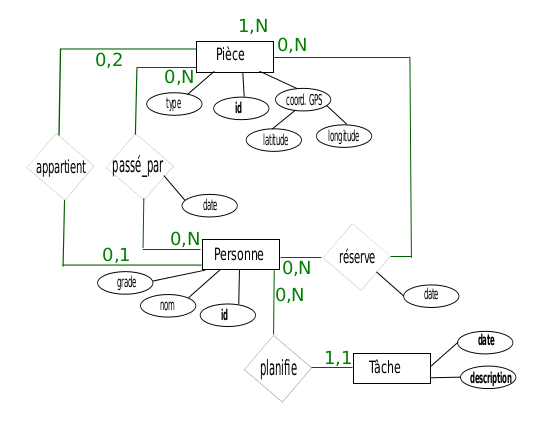
\includegraphics[width=350px]{./images/SchemaEA.png}
	\end{center}
\caption{Schéma EA}
\label{Schéma EA}
\end{figure}

En suivant chaque étape du cours, nous avons obtenu les résultats suivants :

\begin{enumerate}
	\item Passage des entités en relations :
		\begin{itemize}
			\item \code{piece}(idPiece, type, latitude, longitude) : l'attribut composite coord\_GPS est remplacé par ces 2 attributs, latitude et longitude.
			\item \code{personne}(id, nom, grade)
			\item \code{tache}(date, tache) 
		\end{itemize}
	\item Passage des entités faibles en relations : rien à faire puisqu'il n'y a pas d'entités faibles
	\item Association binaire 1,1 par clés étrangères :
		\begin{itemize}
			\item \code{piece}(idPiece, type, latitude, longitude) : schéma inchangé
			\item \code{personne}(id, nom, grade) : schéma inchangé
			\item \code{tache}(date, tache, id) : ajout de la clé étrangère id, clé de \code{personne} car il y a une cardinalité 1,1
		\end{itemize}
	\item Assocations binaires M,N :
		\begin{itemize}
			\item \code{piece}(idP, type, latitude, longitude) : schéma inchangé
			\item \code{personne}(idPers, nom, grade) : schéma inchangé
			\item \code{tache}(date, tache, idPers) : schéma inchangé
			\item \code{appartient}(idP, idPers) : création de la relation \code{appartient} à cette étape
			\item \code{passepar}(idP, idPers, date) : création de la relation \code{passepar} à cette étape
			\item \code{reservation}(idP, idPers, date) : création de la relation \code{reservation} à cette étape
		\end{itemize}
	\item Il n'y a pas d'attributs multi-valués ni d'association n-aire.
\end{enumerate}

\subsection{Critique du modèle Entité-Relationnel}
	On remarque que le modèle semble bien conçus et n'engendre aucun problème. Par exemple, il n'y a pas de redondances des données, les informations concernant les personnes (nom, grades) ou les pièces (coordonées, type) ne sont pas répétées pour chaque reservation de salle avec ce modèle et le modèle relationnel qui en découle. 
	
	De ce fait, les mises à jour n'induisent pas d'incohérence : si le nom de la personne est modifié, il ne faut pas le changer à différents endroits pour rester cohérent.\\
	
	On remarque également l'absence d'anomalie de suppression. Une personne peut n'être concernée par aucune association, c'est-à-dire qu'elle ne possède pas de bureau, n'est passée par aucune pièce et n'a rien reservé, on peut tout de même conserver les informations la concernant puisqu'elles sont séparées.


		\section{Noms des tables et des attributs}
		Retrouvez ci-dessous la description des tables utilisées dans ce projet ainsi que leurs attributs.

\subsection{Table piece}
\begin{itemize}
	\item \code{idP} : l'identifiant de la pièce.
	\item \code{type} : le type de la pièce. Les valeurs possibles sont : Bureau, Salle de Cours, Autre.
	\item \code{gps\_lat} : latitude de la pièce.
	\item \code{gps\_long} : longitude de la pièce.
\end{itemize}

\subsection{Table personne}
\begin{itemize}
	\item \code{idPers} : l'identifiant de la personne.
	\item \code{nom} : le nom de la personne.
	\item \code{grade} : le grade de la personne. Les valeurs possibles sont : Etudiant, MCF, PU, BIATOSS, PE
\end{itemize}

\subsection{Table tache}
\begin{itemize}
	\item \code{date} : la date de la tâche.
	\item \code{tache} : la description de la tâche planifiée. Les valeurs possibles sont : Enseignement, Recherche, Réunion.
	\item \code{idPers} : l'identifiant de la personne.
\end{itemize}

\subsection{Table appartient}
\begin{itemize}
	\item \code{idP} : l'identifiant de la pièce.
	\item \code{idPers} : l'identifiant de la personne.
\end{itemize}

\subsection{Table passePar}
\begin{itemize}
	\item \code{idP} : l'identifiant de la pièce.
	\item \code{idPers} : l'identifiant de la personne.
	\item \code{date} : la date du passage.
\end{itemize}

\subsection{Table reservation}
\begin{itemize}
	\item \code{idP} : l'identifiant de la pièce.
	\item \code{idPers} : l'identifiant de la personne.
	\item \code{date} : la date de la réservation.
\end{itemize}

\vspace{30px}
Les types des attributs peuvent être retrouvés dans le fichier de création des tables : \code{src/SQL/creation.sql}.

		\section{Choix des clés et des contraintes}
		\subsection{Choix des clés}
Pour les tables \textbf{\code{piece}} et \textbf{\code{personne}} on choisit comme clés primaires \code{idP} et \code{idPers} car ils identifient clairement une pièce ou une personne. On choisit ces attributs comme clés primaires et ces attributs seront utilisés comme clés étrangères dans d'autres tables.\\

Pour les tables \textbf{\code{passePar}} et \textbf{\code{reservation}} nous devons définir comme clé primaire les attributs \code{idP}, \code{idPers} et \code{date} car on référence un événement qui se déroule à une date et qui lie une pièce à une personne. Il est nécessaire d'utiliser les 3 attributs comme clés primaires dans ces deux tables pour identifier un tuple. Cette tables sont des tables de liaison donc on utilise les clés primaires des tables que l'on veut lier.\\

Pour la table \textbf{\code{tache}}  nous devons définir comme clé primaire les attributs \code{tache}, \code{idPers} et \code{date} car on référence une tache planifiée par une personne à une date. L'explication est très similaire au paragraphe précédent. Cette tables sont des tables de liaison donc on utilise les clés primaires des tables que l'on veut lier.\\

Enfin, pour la table \textbf{\code{appartient}} on choisit comme clé primaire les attributs \code{idP} et \code{idPers} pour permettre de dire qu'une personne est propriétaire d'une pièce. Cette table est une table de liaison donc on utilise les clés primaires des tables que l'on veut lier.


\subsection{Choix des contraintes}
Parmi les contraintes qu'il nous a semblé primordiale de respecter, la première était l'unicité des clés primaires qui devaient églament être non-nulles. C'est pourquoi pour chaque table nous avons renseigné les clés primaires décrites précédemment par \code{PRIMARY KEY}.\\

Nous avons également veillé au respect des contraintes pour les clés étrangères en utilisant \code{references}. Ainsi, pour la table \code{tache}, nous avons indiqué que l'attribut \code{idPers} était une clé étrangère faisant référence à \code{idPers}, la clé de \code{personne}. De même, pour les tables \code{appartient}, \code{passePar} et \code{reservation}, \code{idP} et \code{idPers} sont deux clés étrangères correspondant respectivement aux clés primaires de \code{piece} et \code{personne}.\\

Concernant la table appartient, seules les personnes dont le grade est \code{MCF}, \code{PU} ou \code{BIATOSS} peut posséder une pièce et la pièce possedée doit être de type \code{Bureau}. Afin de vérifier que ces conditions sont bien respectées nous avons créé le trigger \code{triggerAppartient} qui appelle la fonction \code{testAppartient()}. Cette fonction vérifier que la personne n'est pas de type \code{Etudiant} ou \code{PE} et que la pièce est bien de type \code{Bureau} à l'aide d'un si.\\


La table reserve necessite plusieurs contraintes : seules les personnes dont le grade est \code{MCF}, \code{PU} ou \code{BIATOSS} peuvent reserver une salle, il faut que la salle reservée est un type cohérent avec le grade de la personne et la tâche pour laquelle elle est reservée et la salle ne doit pas faire l'objet d'une autre réservation pour la même date. Nous vérifions chacune de ces contraintes à l'aide du trigger \code{triggerReservation}, correspondant à la fonction \code{testReservation()}

Dans un premier temps, cette fonction vérifie que la personne pour laquelle on veut faire la reservation est bien de grade \code{MCF}, \code{PU} ou \code{BIATOSS} à l'aide d'un si.

Elle compte ensuite le nombre de reservation pour cette salle à cette date afin de vérifier que ce nombre est nul et qu'on peut donc bien reserver la salle.

Dans une dernière partie, la fonction regarde si la personne a déjà planifié une tâche à cette date et si c'est la cas, que le type de la salle est bien cohérent avec celui de la tâche.\\

Enfin, un dernier trigger, \code{triggerTache}, associé à la fonction \code{testTache()}, vérifie les contraintes concernant la table Tache, c'est-à-dire que la personne n'est pas de type \code{PE} et que la tâche planifiée est bien cohérente avec le grade de la personne.


		\section{Difficultés rencontrées}  
			\subsection{Serveur PostgreSQL local}
			Nous avons dû installer sur nos ordinateurs personnels PostgreSQL en client et en serveur pour pouvoir développer rapidement. En effet, nous ne voulions pas à avoir à monter des tunnels SSH vers l'INSA de Rouen pour travailler sur le serveur PostgreSQL de l'INSA.\\

L'installation de PostgreSQL sous Ubuntu est facile mais la configuration est un petit peu plus délicate. Nous avons utilisé la documentation en ligne de PostgreSQL et quelques forums trouvés grâce à des moteurs de recherche. Nous avons mis un petit peu de temps à changer le mot de passe de l'utilisateur par défaut, créer notre utilisateur \code{grtt6}, créer une base du même nom et définir les droits adéquats dessus. Mais maintenant nous maîtrisons parfaitement la procédure ! Une fois ceci effectué nous n'avons plus eu aucun problème et nous avons pu écrire nos scripts SQL et les tester sans problème.
			
			\subsection{Rapport d'intrusion}
			La fonctionnalité nous ayant posé le plus de difficultés a été le rapport d'intrusion. En effet, après avoir écrit une première version de la fonction \code{estIntru} qui nous paraissait cohérente, nous avons constaté que les résultats obtenus ne correspondaient pas à ceux de l'exemple d'utilisation.

\inputminted[tabsize=4,linenos,fontsize=\small]{sql}{code/1.sql}

Les résultats que nous étions censés obtenir avec la première version du fichier d'exemple d'exécution étaient :
\begin{center}
	\begin{tabular}
		{| l |	c |	c |} \hline
		2014-01-20 & s3 & Amanda Maire \\ \hline
		2014-01-20 & s3 & Mousse Line \\ \hline
		2014-01-20 & s2 & Mousse Line \\ \hline
		2014-01-13 & s1 & Louis Dort \\ \hline
		2014-05-10 & s7 & Geo Graff \\ \hline
		2014-01-22 & s1 & Albert Gamotte \\ \hline
		2014-01-20 & s3 & Amanda Maire \\ \hline
		2014-01-20 & s3 & Mousse Line \\ \hline
	\end{tabular}
\end{center}

Mais nous obtenions les résultats suivant :
\begin{center}
	\begin{tabular}
		{| l |	c |	c |} \hline
		2014-01-13 & s1 & Laure Aidubois \\ \hline
		2014-01-22 & s1 & Albert Gamotte \\ \hline
		2014-05-10 & s7 & Geo Graff \\ \hline
		2014-01-13 & s1 & Louis Dort \\ \hline
		2014-01-20 & s3 & Mousse Line \\ \hline
		2014-01-20 & s3 & Amanda Maire \\ \hline
	\end{tabular}
\end{center}



Le rapport d'intrusion résultant d'une fonction assez compliquée, il nous était très difficile de trouver la source de ces différences et d'expliquer nos erreurs en regardant simplement les tables. Nous avons donc été amenés à écrire une requête SQL nous permettant d'avoir une vue d'ensemble et de mieux voir quels tuples nous manquaient, quels tuples nous avions en trop et pourquoi.\\

Nous avons donc utilisé la requête :
\inputminted[tabsize=4,linenos,fontsize=\small]{sql}{code/2.sql}

qui nous a affiché les résultats suivants :

\begin{center}
	\begin{tabular}
		{| l |	c |	c | c | c | c |} \hline
		nom       & idpers &  grade   &    date    & idp & proprietaire \\ \hlineGras
		 Lance Pierre   & p1      & MCF      & 2014-01-12 & s1  & p1 \\ \hline
		 Lance Pierre   & p1     & MCF      & 2014-01-12 & s1  & p2 \\ \hline
		 Laure Aidubois & p2     & MCF      & 2014-01-13 & s1  & p1 \\ \hline 
		 Laure Aidubois & p2     & MCF      & 2014-01-13 & s1  & p2 \\ \hline
		 Louis Dort     & p7     & Etudiant & 2014-01-13 & s1  & p1 \\ \hline
		 Louis Dort     & p7     & Etudiant & 2014-01-13 & s1  & p2 \\ \hline
		 Bruno Zieuvair & p5     & PE       & 2014-01-14 & s1  & p1 \\ \hline
		 Bruno Zieuvair & p5     & PE       & 2014-01-14 & s1  & p2 \\ \hline
		 Mousse Line    & p9     & Etudiant & 2014-01-20 & s2  & p3 \\ \hline
		 Albert Gamotte & p3     & PU       & 2014-01-20 & s2  & p3 \\ \hline
		 Amanda Maire   & p10    & Etudiant & 2014-01-20 & s3  & p4 \\ \hline
		 Mousse Line    & p9     & Etudiant & 2014-01-20 & s3  & p4 \\ \hline
		 Albert Gamotte & p3     & PU       & 2014-01-22 & s1  & p1 \\ \hline
		 Albert Gamotte & p3     & PU       & 2014-01-22 & s1  & p2 \\ \hline
	\end{tabular}
\end{center}

Ainsi nous avons pu voir que \textit{2014-01-13 | s1 | Laure Aidubois}, considéré comme un intru par notre fonction, était la deuxième propriétaire de la salle s1 dans laquelle elle se trouve et ne devait donc pas être considéré comme intru. De ce fait \textit{2014-01-13 | s1 | Louis Dort}, présent au même moment, ne devait pas être considéré comme un intru non plus.

Nous en avons conclu que notre fonction ne gérait pas les propriétaires multiples pour un même bureau.\\

De même, nous avons constaté que le tuple \textit{2014-05-10 | s7 | Geo Graff}, présent dans notre rapport d'intrusion, n'apparaissait même pas dans les résultats que nous obtenions, et ceci pour une raison simple : la salle s7 étant une salle de cours, elle ne possède pas de propriétaire.

Nous avons donc pu voir que notre fonction ne gérait pas les pièces autres que les bureaux, qui ne possèdent pas de propriétaires et qui ne devaient donc pas être prises en compte dans le rapport d'intrusion.\\

À l'aide de cette requête nous avons donc pu repérer nos erreurs et effectuer les modifications nécessaires pour obtenir des résultats cohérents. Nous avons ainsi pu corriger notre fonction \code{estIntru} dont le code est le suivant :

\inputminted[tabsize=4,linenos,fontsize=\small]{sql}{code/3.sql}

	\chapter{Ce qui aurait pu être fait}
		\section{Contraintes supplémentaires}
		\subsection{Contraintes sur les dates}
Il aurait été bien d'avoir des contraintes empêchant de planifier des tâches ou de réserver des salles dans le passé, c'est-à-dire pour une date antérieure à la date actuelle. De plus, il n'est actuellement pas possible de planifier des tâches ou des réservations de manière plus précise que pour une journée, ce qui est assez irréaliste. Il aurait été bien de pouvoir planifier pour une intervalle de temps, avec une date de début et une date de fin. 

\subsection{Contraintes sur les réservations}
Actuellement il est possible de réserver une salle même si on n'a pas définit de tâche, ce qui n'est pas optimal pour le suivi du planning des personnes de l'université.

		\section{Report des exceptions dans l'application}
		Nous avons mis en place plusieurs triggers de vérification de contraintes d'intégrité complexes lors de la création de notre base de données. Ces triggers lèvent des exceptions lorsque l'on tente de faire une mise à jour qui viole les contraintes d'intégrité. Lorsque l'on tente de faire une mise à jour qui viole une contrainte d'intégrité en ligne de commande dans le terminal, l'exception levée par PostgreSQL est affichée directement dans le terminal.\\

Nous voulions pouvoir reproduire ce comportement pour les mises à jour ne respectant pas les contraintes d'intégrité effectuées depuis notre application. Après une longue recherche, nous avons réalisé que la directive \code{EXEC SQL WHENEVER sqlerror sqlprint;} ne s'appliquait qu'à la fonction où elle se trouvait. Nous avons donc déplacé cette directive au début du programme, en dehors d'une fonction pour avoir une portée globale.

	\chapter{Répartition du travail et conclusion}
		\section{Répartition du travail}
Retrouvez dans le tableau ci-dessous comment nous avons réparti entre nous les différentes fonctionnalités à réaliser pour mener ce projet : 
\begin{center}
	\begin{tabular}
	{| l ||	c |	c |} \hline
		Tâche & Manon Ansart & Antoine Augusti \\ \hline \hline
		\textbf{Conception de la base de données} & & \\ \hline
		Passage au modèle relationnel & \checkmark & \checkmark \\ \hline
		Création des tables & & \checkmark \\ \hline
		Insertion des données & \checkmark &  \\ \hline
		Création des droits & \checkmark &  \\ \hline
		Création des index & & \checkmark \\ \hline
		Création des fonctions & \checkmark &  \\ \hline
		Création des vues & & \checkmark \\ \hline
		Script de suppression & \checkmark &  \\ \hline
		\hlineGras 
		\textbf{Application de gestion} & & \\ \hline
		Ajout d'une personne & \checkmark &  \\ \hline
		Suppression d'une personne & \checkmark &  \\ \hline
		Réservation d'une salle & & \checkmark \\ \hline
		Lieux visités par une personne & \checkmark &  \\ \hline
		Rapport d'activité d'une personne & & \checkmark \\ \hline
		Rapport d'intrusion & & \checkmark \\ \hline
		\hlineGras 
		\textbf{Rapport} & & \\ \hline
		Rédaction du rapport & \checkmark & \checkmark \\ \hline
		\hlineGras 
		\textbf{Gestionnaire de versions} & & \\ \hline
		Mise en place de Git &  & \checkmark \\ \hline
		\hlineGras 
	\end{tabular}
\end{center}

	\chapter{Annexes}
		\section{Code source SQL}
			\subsection{creation.sql}
			\inputminted[tabsize=4,linenos,fontsize=\small]{sql}{../src/SQL/creation.sql}

			\subsection{suppression.sql}		
			\inputminted[tabsize=4,linenos,fontsize=\small]{sql}{../src/SQL/suppression.sql}

		\section{Code source C}
			\subsection{appliUniv.pgc}
			\inputminted[tabsize=4,linenos,fontsize=\small]{sql}{../src/C/appliUniv.pgc}


\end{document}